\documentclass[a4paper, twocolumn]{jarticle}
%\documentclass[uplatex]{jsarticle}
\usepackage[dvipdfmx]{graphicx}
\usepackage{algorithmic,algorithm}
\usepackage{float}

%\usepackage[dvips]{color} 
%\usepackage{ascmac}
%\usepackage{verbatim}
\usepackage{setspace}
\usepackage[top=20mm,bottom=20mm,left=23mm,right=23mm]{geometry}
\makeatletter
\def\section{\@startsection{section}{1}{\z@}%
 {.1\Cvs \@plus.1\Cdp \@minus.1\Cdp}%
 {.1\Cvs \@plus.1\Cdp}%
 {\normalfont\normalsize\bfseries}}
\renewcommand{\thesection}{\arabic{section}.}
\renewcommand{\thesubsection}{\arabic{section}.\arabic{subsection}}
\def\subsection{\@startsection{subsection}{1}{\z@}%
 {.1\Cvs \@plus.1\Cdp \@minus.1\Cdp}%
 {.1\Cvs \@plus.1\Cdp}%
 {\normalfont\normalsize\bfseries}}


\def\@maketitle {
	\begin{center}
		\fontsize{14pt}{0pt}\selectfont
                {\bf \@title{}}
	\end{center}
	\vspace{1pt}
	\begin{flushleft}
		\@author{指導教員 福田浩章 }
		\hfill{川部勝也}
	\end{flushleft}
\vspace{0.3cm}
}

%\makeatother

%\makeatletter


\renewcommand{\baselinestretch}{0.95}


\pagestyle{empty}
\makeatother

\begin{document}
\title{ロバスト性を有するWSN用ルーティングアルゴリズムの提案と実装}
\date{}
\maketitle
\thispagestyle{empty} 

%%%%%%%%%%%%%%%%%%%%%%%%%%%%%%%%%%%%%%%%
%%背景
%%%%%%%%%%%%%%%%%%%%%%%%%%%%%%%%%%%%%%%%
\section{背景}
IoTの普及に伴い, 無線センサネットワーク(WSN:Wiress Sensor Network)は自然科学, 医療, 軍事など様々な分野で利用されている.
WSNは周囲の環境情報を収集し, その情報を一定間隔でベースステーションに送信する.
この場合, ベースステーション付近のノードにトラフィックが集中してバッテリーの消費が多くなる.
ベースステーションに繋がるノードがダウンすると, それ以降のデータはベースステーションに送信されなくなる.
この問題を解決するために, Distributed Hash Table(DHT)\cite{DHT}をWSN上で構築し, 負荷を分散する研究がある\cite{DHT-on-WSN-survey}.
DHTは中央サーバが存在せず, 純粋なP2P型のネットワークを実現することができる技術である.
管理するデータの識別子をファイル名やファイル自体からハッシュ関数を用いて算出されるハッシュ値で表現する.
多くのDHTはO(logN)で探索が可能で, 負荷が一つのノードに偏らない.
Chord\cite{Chord}はDHTの一種で, 単純なアルゴリズムでデータの存在可否を確実に保証する. 
Chordは識別子が時計回りに増加していく論理的なリング状のネットワークを導入している.
WSNでは物理的な距離が離れているとパケットが届かず, Chordのリング状ネットワークを適用する際にはこの問題を考慮する必要がある.
%%%%%%%%%%%%%%%%%%%%%%%%%%%%%%%%%%%%%%%
%% 研究手順
%%%%%%%%%%%%%%%%%%%%%%%%%%%%%%%%%%%%%%%%
\section{関連研究}
\subsection{CSN}
Chordは論理的なリング状ネットワークを構築するが, リング上でノード同士の距離が近くとも, 物理的な距離が遠い場合もある.
その場合, パケットが届かない可能性があり, データの検索を保証できない.
CSNは物理的に近い距離のノード同士でリングを作り, 階層化することでこの問題を解決している.
しかし, CSNでは管理者がWSNに保存されているデータを検索する前提なので, 最上層のノードからしかデータ検索を行えない.
\subsection{CMSN}
CMSN\cite{CMSN}はCSNをモバイルエージェントの探索用に拡張した研究である.
リングに参加しているノード全てからデータ検索を行えるが, 検索を行ったあとの結果の返信についてはサポートしていない.
さらに, リングの構築には個々のノードがどの位置で, どの階層のリングに属するかを予め決定しておく必要がある.
これは, ノードの配置が限定される上, ノード毎に階層の情報を個別にプログラムする必要があり, 管理者の負担となる.

本研究では, 検索時に経路情報を持たせ, 確実な検索結果の返信を保証し,
リング構築時にノードに階層の情報を持たせず, ノードの配置に応じたリングを構築するルーティングアルゴリズムを提案する.

\section{リング構築アルゴリズム}
\subsection{構築手順}
前提として, ノードが持つ初期情報はWSN全体でのクラスタヘッド, 最上層のリング参加限界数(top\_limit)とする.
ネットワークの構築はクラスタヘッド(N1)がリング構築メッセージをブロードキャストして開始する.
メッセージを受け取ったノードのうち, どのリングにも属していないノードはACKを返す.
N1は受信したACKの中で物理的に最も近いノード(仮にN2とする)をリンク先に選び, その旨をN2に対して通知する.
このメッセージには現在のリングに参加しているノード数, クラスタヘッドの識別子, 所属する階層の深さの情報が含まれる.
自身が所属する階層の深さを level とすると現在参加しているリングの参加限界数(limit)を以下の式(1)(2)で表す.
\begin{eqnarray}
  e = level - 1 \\
  limit = top\_limit / 2^e
\end{eqnarray}
現在のリングに参加しているノード数が参加限界数未満ならば, 同様の手順でリンク先のノードを探索する. 
これを繰り返し, リングに参加するノード数が限界に到達したか, ブロードキャストにACKが返ってこなかった時はリングの構築完了メッセージをクラスタヘッドに送信する.
この時, リングの終端からクラスタヘッドにパケットが届かない可能性がある.
そのため, リングの終端からリング内のクラスタヘッドにパケットを送信する場合のみ, リング内を逆に辿ってパケットを転送することで, パケットの到達を保証する.
リング構築完了のメッセージを受け取ったノードは下層のリングを構築するため以上の手順を繰り返す.
下層のリング構築を完了すると, 同じ階層の隣接しているノードへ下層リング作成のメッセージを送信する.
メッセージを受信すると, 同様に下層のリング構築を開始する.
これを繰り返し最下層のリングまで構築する.
%下層のリング作成を同一階層内で並列で実行しない理由はパケットの輻輳による意図しないパケットの喪失を防ぐためである.

\section{検索後の返信}
リング構築後に検索結果を検索元のノードに返信するためのアルゴリズムについて述べる.
検索時, 返信時のメッセージの構成はハッシュ値, 経路情報, 経路情報のインデックス, 検索結果から成る.
経路情報はノードの識別子を格納する配列であり, 最長はノード総数をN, 階層数をMとした時 2*MlogN となる.
検索後, 結果を格納したノードは経路情報の末尾の識別子を参照し, 識別子のノードに結果メッセージ送信する.
この時, 識別子のノードは物理的に近い距離であることがリングの構築時に保証されているため, パケットが届かないことはない.
メッセージを受け取ったノードはインデックスを参照し, 経路情報の識別子を取得する.
インデックスをデクリメントしてから識別子のノードに同様にメッセージを送信し, 経路情報の先頭のノードまで送信を繰り返す. 

\section{検証, 考察}
検証にはWSN用OSであるContiki\cite{Contiki}と付属するシミュレータ, Coojaを用いた.
検証用プログラムの実装はC言語で行った.
\subsection{リングの構築}
ノードを正方形の領域内にランダムに配置し, 
配置数と領域の大きさを変え, リングの構築をそれぞれ20回行った結果を表1に示す.
全ての実験で現実的な時間内で確実にリングを構築することができた.
リングの参加率がこのような結果となった原因はノードの配置によって図\ref{fig:ring_struct}のように, 
リングに参加しているノードの分布が領域内の局所的な部分に集中してしまい, 早々にリンクするノードを発見できなくなったためと考える.

% 評価表
\begin{table}[htb]
	\scalebox{0.430}{
	\begin{tabular}{|c|c|c|c|c|c|} \hline
		配置数(個) & 最上層参加限界数(個) & 参加率(\%) & リング参加ノード数(個) & 構築時間(分:秒) & 領域(縦*横m) \\ \hline \hline
		72 & 6 & 30 & 75\% & 8:35 & 200*200 \\ \hline
		72 & 8 & 56 & 58\% & 11:42 & 200*200 \\ \hline
		144 & 8 & 56 & 52\% & 12:45 & 300*300 \\ \hline
	\end{tabular}
	}
\end{table}
\begin{figure}[htbp]
	\begin{center}
	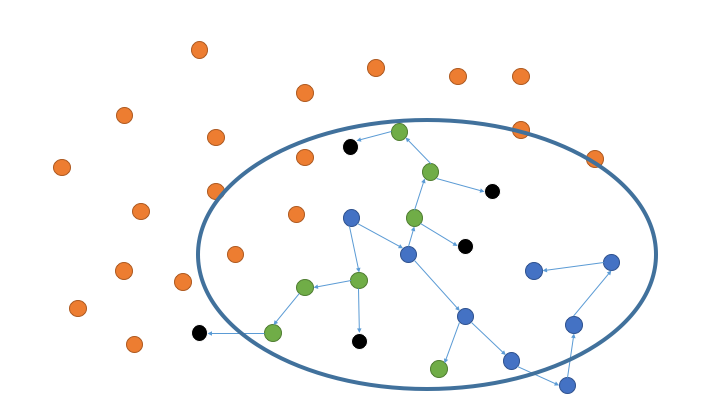
\includegraphics[width=8cm, height=5cm]{ring_struct_failed.png}
	\end{center}
	\caption{リングに参加しているノードの分布}\label{fig:ring_struct}
\end{figure}
\subsection{データ検索}
最上層の参加数を8個, 階層数を3個, 合計参加数を32個のリングを構築し, 全てのノードに10回の検索を行わせた.
この時に検索後の応答パケットに経路情報を持たせ, それを元に返信する場合と, 
近くに検索元のノードが存在しなければ近隣のノードをランダムに一つ選び, 
送信するランダムなマルチホップ通信による応答との消費電力を比較した.
その結果を図\ref{fig:battery_eval}に示す.
消費電力は経路情報をもたせた場合, ランダムなマルチホップに比べて50\%近く削減されている.
WSNは数年に渡る長期間での運用となるため, 消費電力の差は運用期間, ノード数によって非常に大きくなると考えられる.
従って, 結果を検索元のノードに返信するに経路情報を利用するのは有用であると考える.
\begin{figure}[htbp]
	\begin{center}
	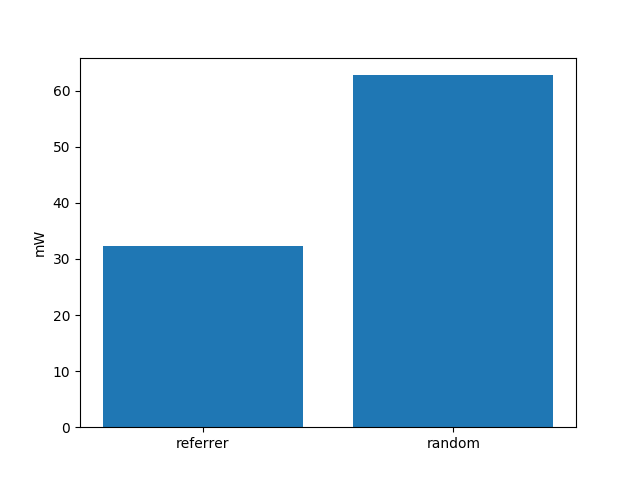
\includegraphics[width=8cm, height=5cm]{battery_eval_2.png}
	\end{center}
	\caption{バッテリー消費量}\label{fig:battery_eval}
\end{figure}

% TODO
% バッテリー消費考察

\section{まとめ}
本研究ではWSNにおいてノードの配置に応じた動的なルーティングアルゴリズムを実現し,
ノードの参加率, 検索結果の返信に経路情報を用いた場合の消費電力を比較することで有効性を調査した.
今後の課題として, リングがWSNの領域内で均等に分散せず, 局所的に形成されてしまったため, 参加率が落ちてしまった.
そこで, リンク時に返信するACKに指向性の情報を持たせ, リングの形を制御することでより多くのノードの参加を実現する必要がある. 
%%%%%%%%%%%%%%%%%%%%%%%%%%%%%%%%%%%%%%%%
%%参考文献
%%%%%%%%%%%%%%%%%%%%%%%%%%%%%%%%%%%%%%%%
\begin{thebibliography}{9}
{\small
% \bibitem{WSN-Surver}
% Khan, Imran, et al. "Wireless sensor network virtualization: A survey." IEEE Communications Surveys and Tutorials 18.1 (2016): 553-576.
\bibitem{DHT-on-WSN-survey}
Thanh, Vinh Vu, et al. "A survey of routing using dhts over wireless sensor networks." Proceedings of The 6th international conference on information technology and applications (ICITA 2009). 2009.
\bibitem{DHT}
江崎浩: ''P2P(ピア・ツー・ピア)教科書'', インプレスR\&D (2008-1)
\bibitem{CSN}
Ali {\em et al.}: CSN: A network protocol for serving dynamic queries in large-scale wireless sensor networks, In {\em Proceeding of the Second Annual Conference on Communication Networks and Services Research}, 2004, pp.165-174.
\bibitem{CMSN}
Fukuda, Hiroaki, Paul Leger, and Keita Namiki. "CMSN: An Efficient and Effective Agent Lookup for Mobile Agent Middleware." J. UCS 22.8 (2016): 1072-1096.
\bibitem{SHA-1}
Xiaoyun Wang, et al. Finding Collisions in the Full SHA-1, Crypto 2005
\bibitem{Chord}
Stoica, Ion, et al. "Chord: A scalable peer-to-peer lookup service for internet applications." ACM SIGCOMM Computer Communication Review 31.4 (2001): 149-160.
\bibitem{Contiki}
Dunkels, Adam, Bjorn Gronvall, and Thiemo Voigt. "Contiki-a lightweight and flexible operating system for tiny networked sensors." Local Computer Networks, 2004. 29th Annual IEEE International Conference on. IEEE, 2004.
}
\end{thebibliography}
\end{document}
